% docs/white_paper_skeleton.tex
\documentclass[11pt]{article}
\usepackage[margin=1in]{geometry}
\usepackage{amsmath,amssymb,amsthm}
\usepackage{graphicx}
\usepackage{hyperref}
\usepackage{authblk}

\title{A Minimal Substrate for Locality, Entanglement Geometry, and Error Protection:\\
Towards a Practical Theory-of-Everything Scaffold}

\author[1]{Your Name}
\affil[1]{Your Affiliation}

\date{\today}

\begin{document}
\maketitle

\begin{abstract}
We introduce a minimal computational substrate that unifies (i) locality and finite propagation (QCA/Lieb--Robinson), (ii) area-law entanglement geometry (minimal cuts $\gamma_A$), and (iii) quantum error-correction feasibility (Knill--Laflamme). We provide open-source tests and figures demonstrating each pillar and their integration.
\end{abstract}

\section{Axioms (Plain-Language)}
\begin{enumerate}
  \item \textbf{Local updates, finite speed:} interactions are strictly local, implying a maximum propagation speed.
  \item \textbf{Entanglement follows minimal boundaries:} correlations across a region scale with the smallest boundary you must cut.
  \item \textbf{Information is redundantly encodable:} with the right patterns, information survives local erasures.
\end{enumerate}

\section{Model Substrate}
We represent degrees of freedom on a graph $G$ with uniform bond dimension $\chi$. A local reversible update (split-step QCA) captures finite-speed dynamics. Entanglement entropy proxy for a boundary region $A$ is $S(A)=|\gamma_A|\log_2\chi$.

\section{Results}
\subsection{Area-law scaling}
\paragraph{Path and ring.} Figure~\ref{fig:path}--\ref{fig:ring} show $S(A)$ vs region size $|A|$ for chains and rings. Rings generically cut two edges, yielding $\approx 2\log_2\chi$ for $0<|A|<N$.

\begin{figure}[h]
  \centering
  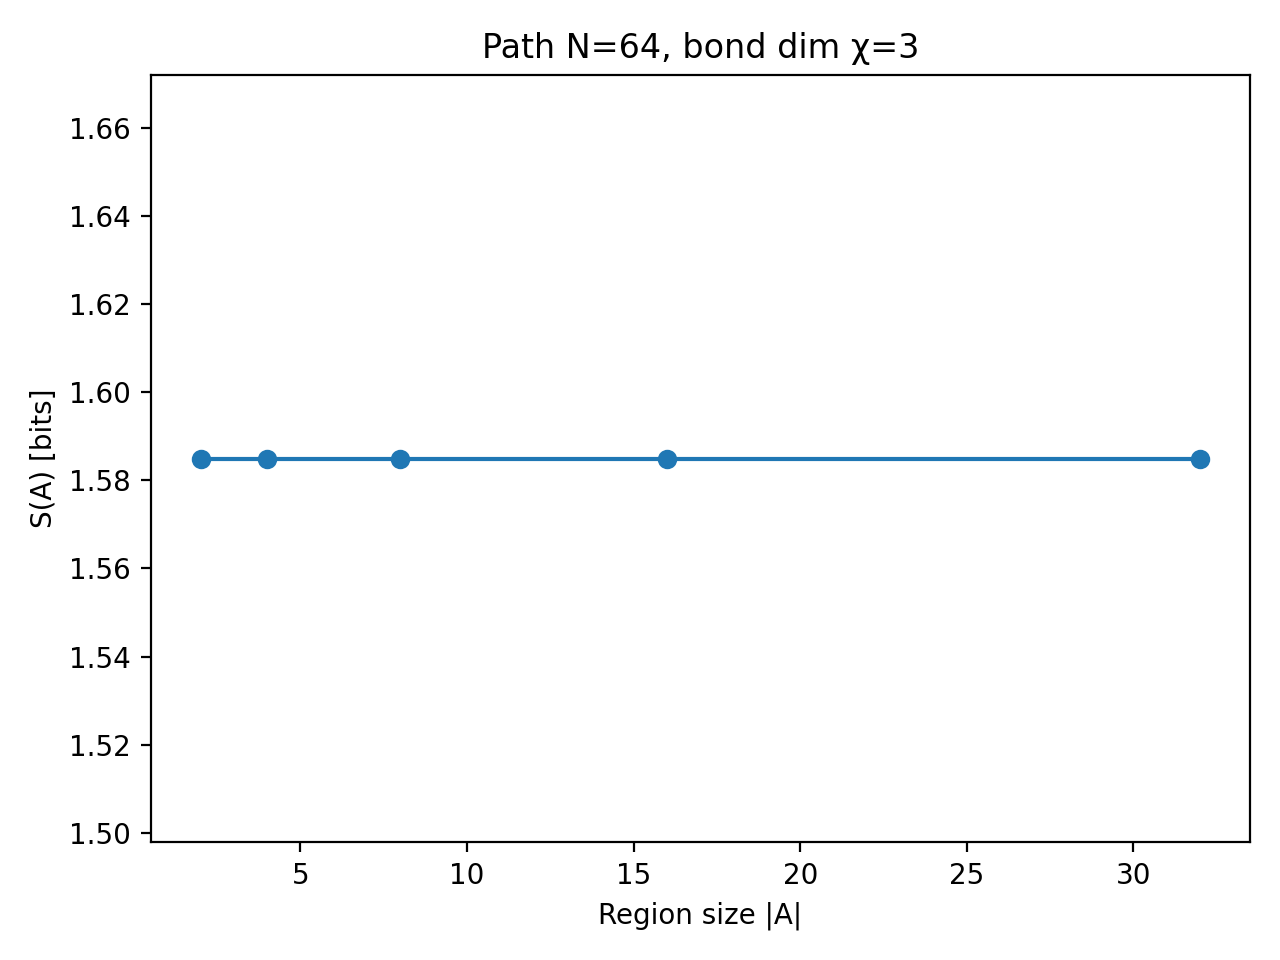
\includegraphics[width=.7\textwidth]{../outputs/figs/entropy_path_N64_chi3.png}
  \caption{Area-law proxy on a path (example).}
  \label{fig:path}
\end{figure}

\begin{figure}[h]
  \centering
  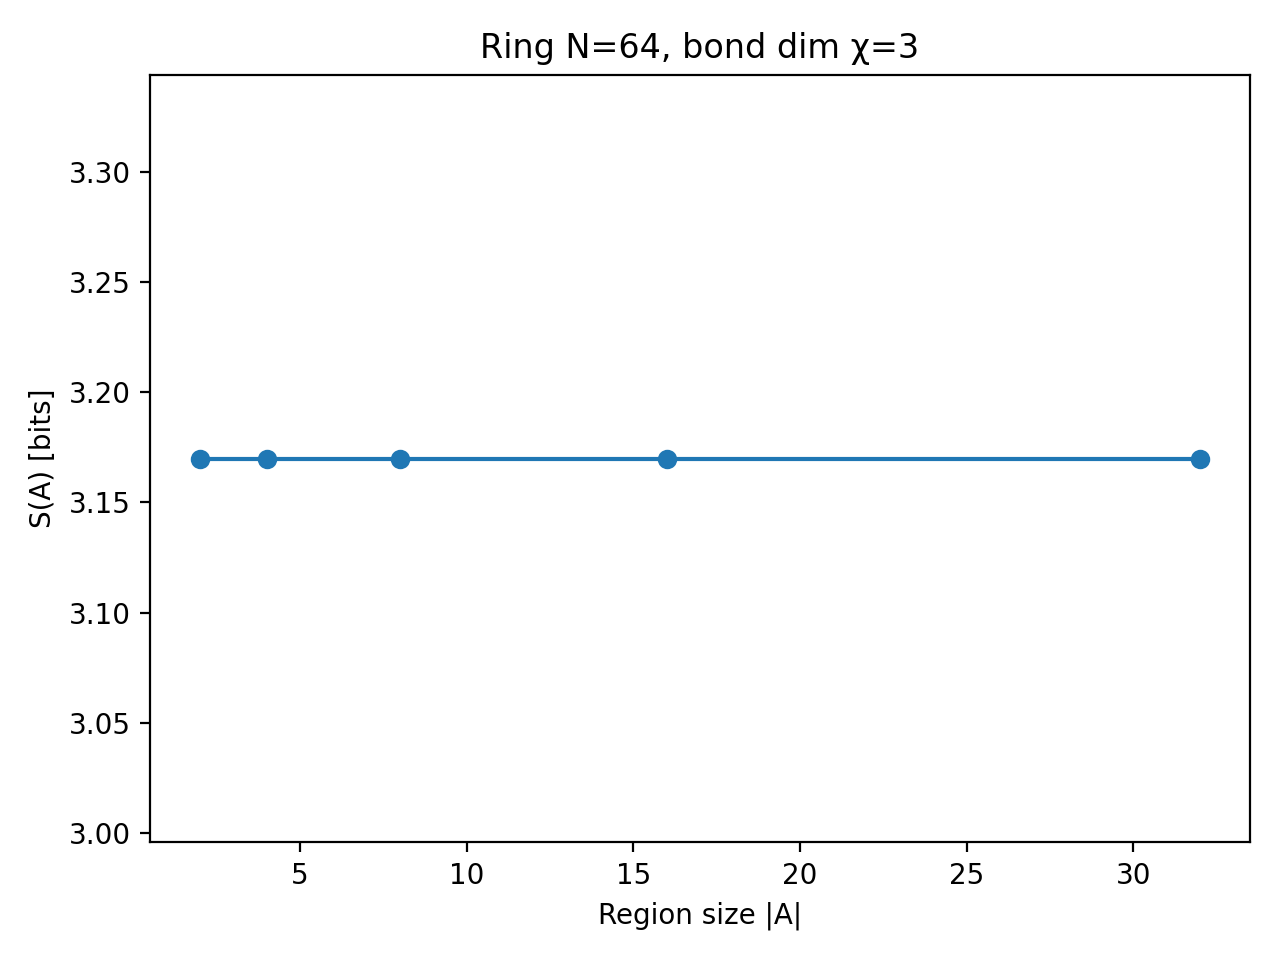
\includegraphics[width=.7\textwidth]{../outputs/figs/entropy_ring_N64_chi3.png}
  \caption{Area-law proxy on a ring (example).}
  \label{fig:ring}
\end{figure}

\paragraph{Random graphs.} On Erdős–Rényi graphs, the proxy scales monotonically with $\chi$ and grows with region size, see Fig.~\ref{fig:er}.

\begin{figure}[h]
  \centering
  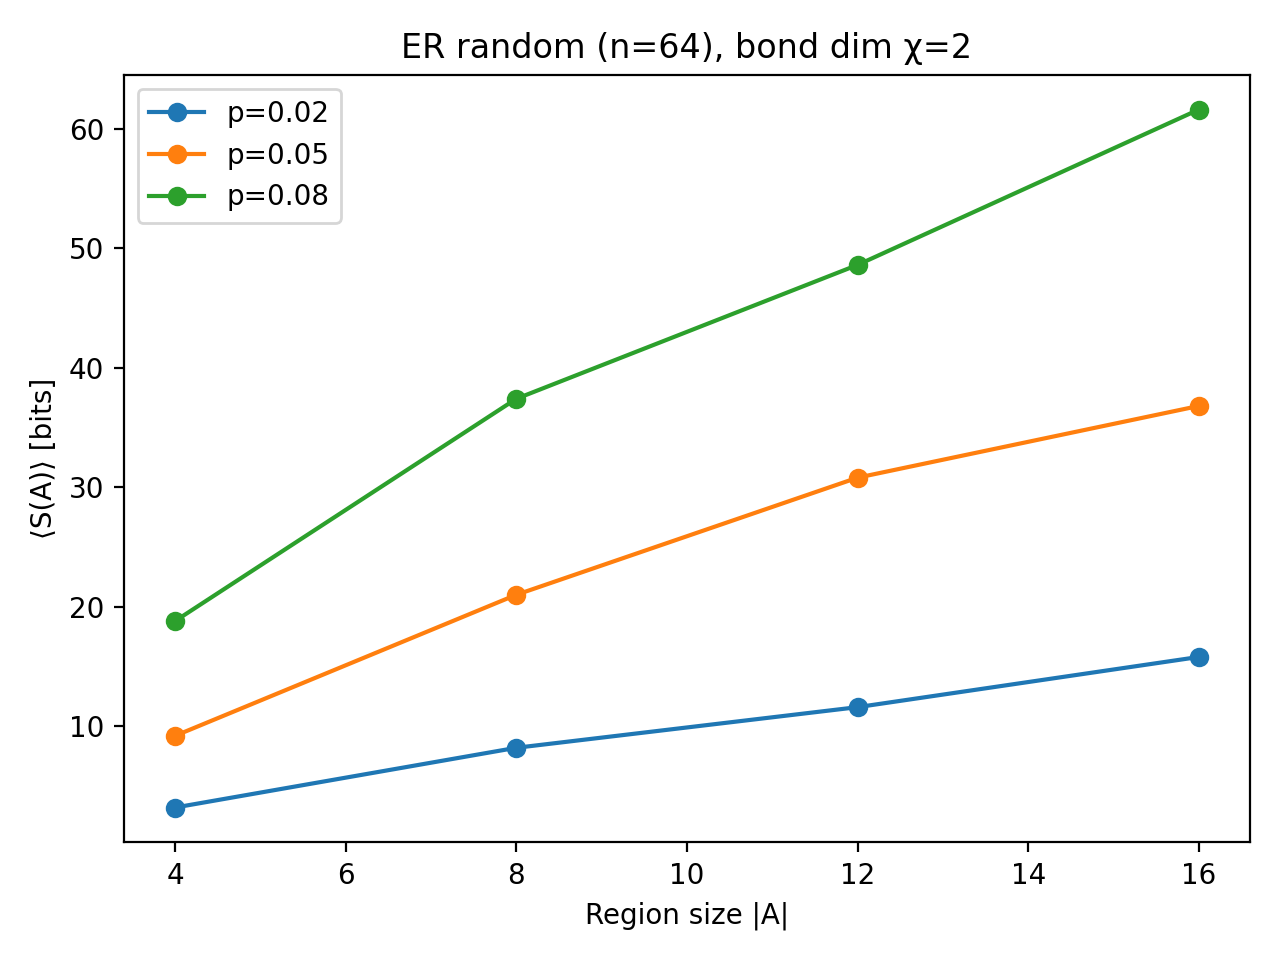
\includegraphics[width=.7\textwidth]{../outputs/figs/entropy_er_random_n64_chi2.png}
  \caption{Average $S(A)$ on ER graphs (example aggregate).}
  \label{fig:er}
\end{figure}

\subsection{Lieb--Robinson velocity}
We bound operator spread without $2^N$ vectors via support growth. Fig.~\ref{fig:lr} shows a linear lightcone radius and a stable effective velocity.

\begin{figure}[h]
  \centering
  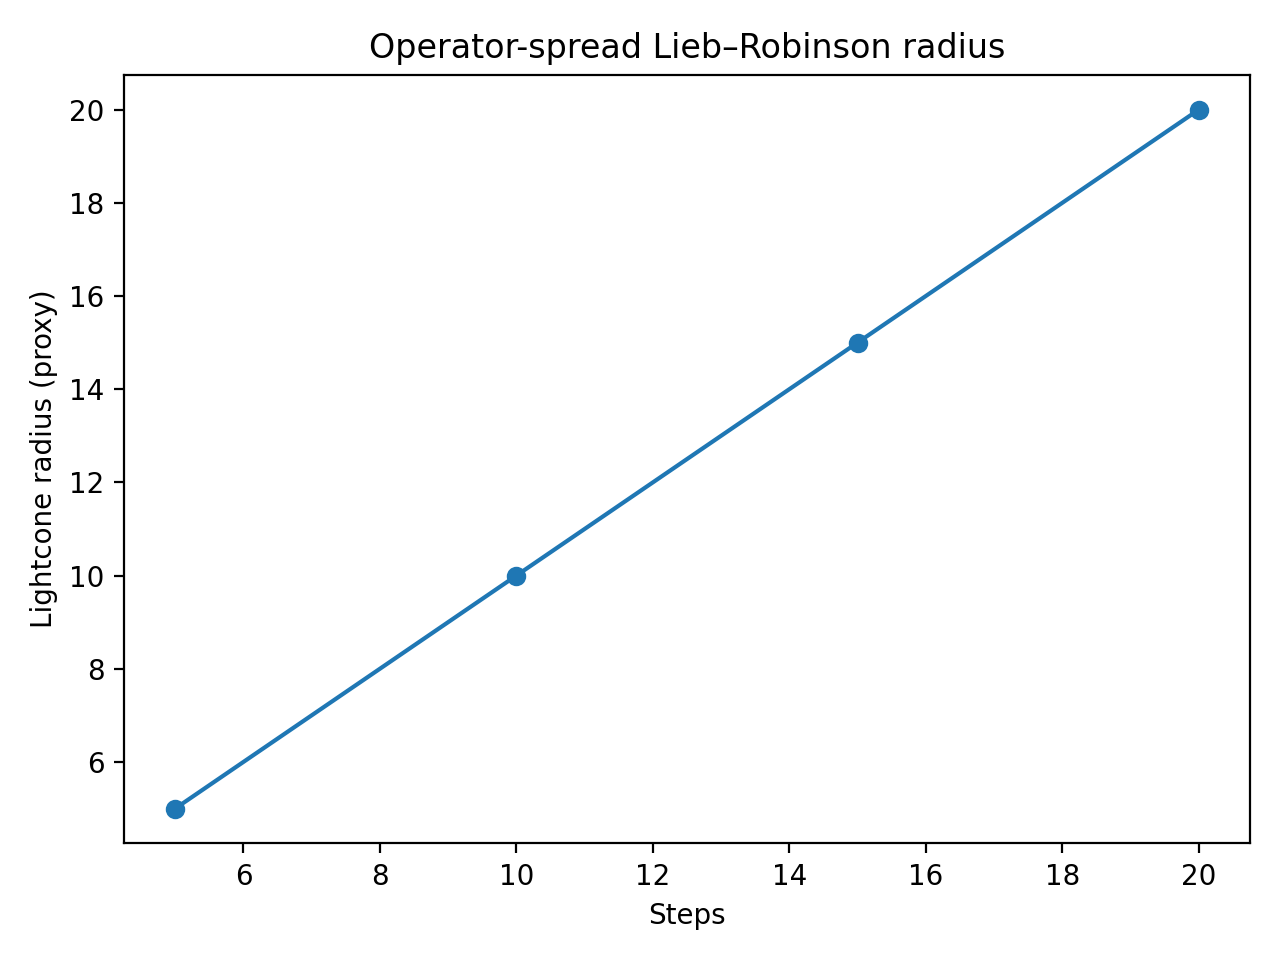
\includegraphics[width=.7\textwidth]{../outputs/figs/lr_radius.png}
  \caption{Operator-spread radius vs steps.}
\end{figure}

\begin{figure}[h]
  \centering
  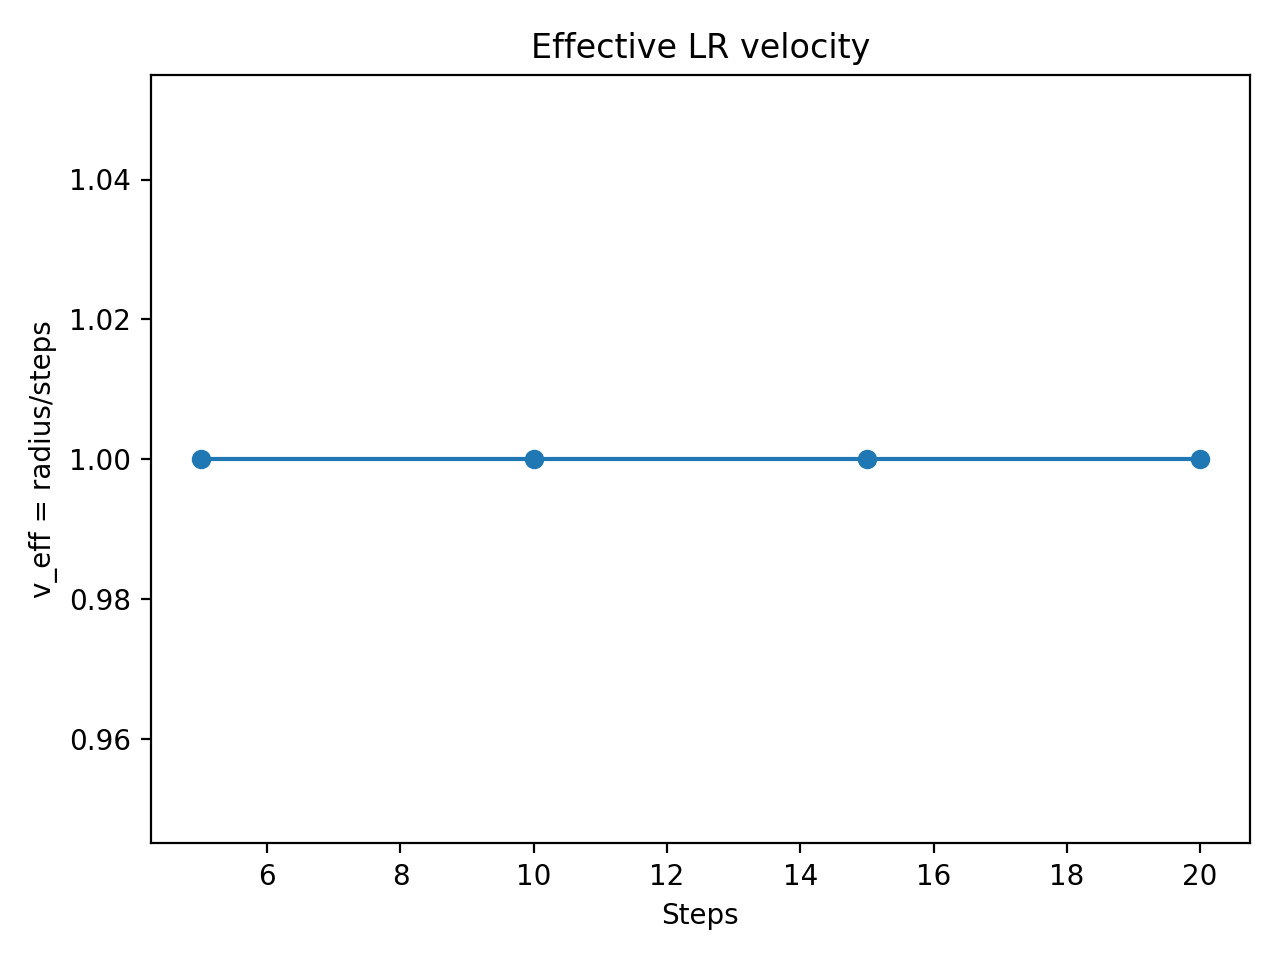
\includegraphics[width=.7\textwidth]{../outputs/figs/lr_velocity.png}
  \caption{Effective Lieb--Robinson velocity $v_{\mathrm{eff}}$.}
  \label{fig:lr}
\end{figure}

\subsection{Knill--Laflamme feasibility}
We map success rates as a function of $(d_{\text{in}}, d_{\text{out}}, w)$. See Fig.~\ref{fig:kl} for representative slices.

\begin{figure}[h]
  \centering
  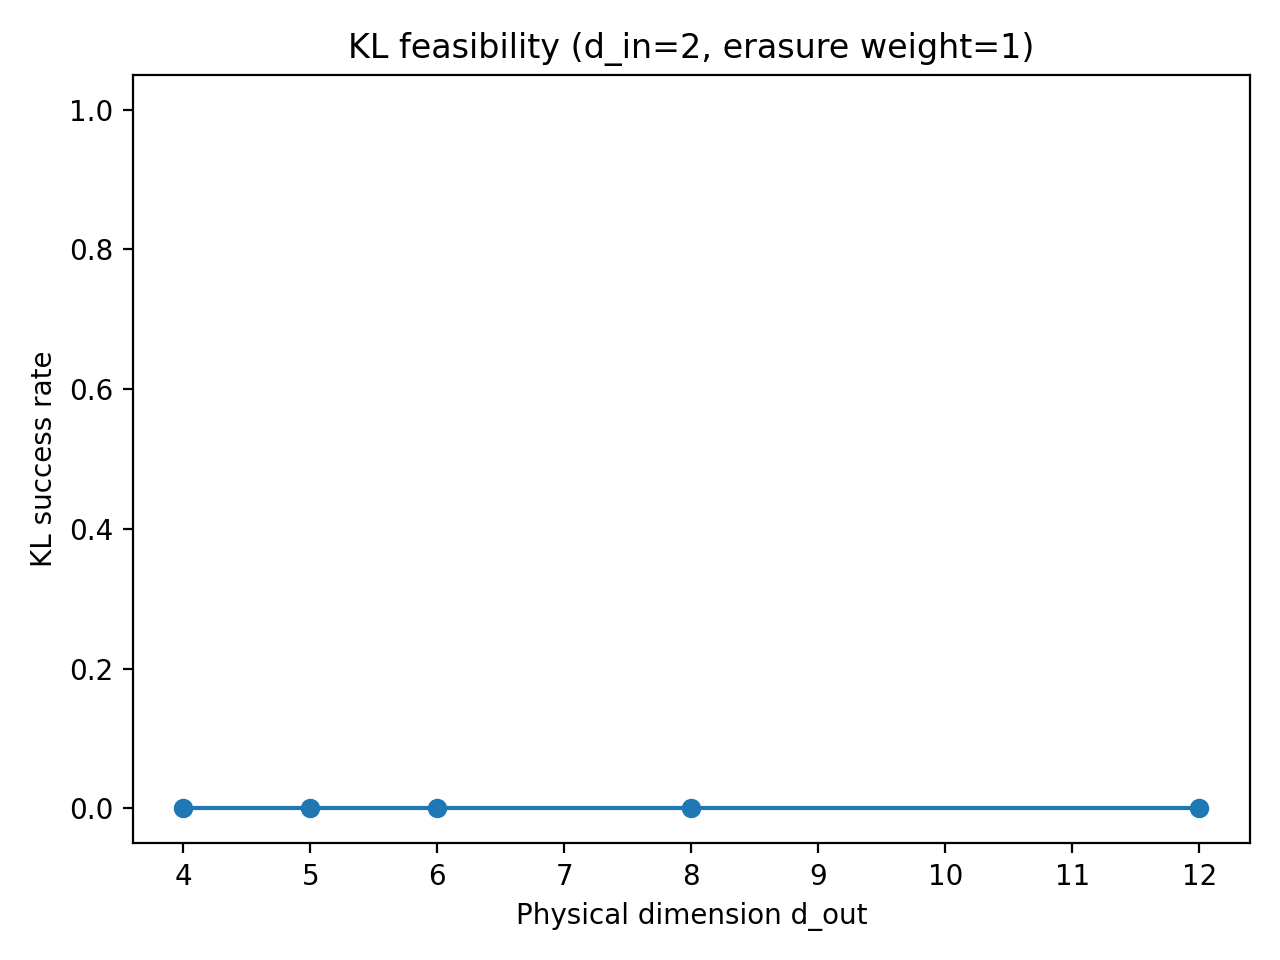
\includegraphics[width=.7\textwidth]{../outputs/figs/kl_success_din2_w1.png}
  \caption{KL success rate vs physical dimension for $d_{\text{in}}=2$, weight $w=1$.}
  \label{fig:kl}
\end{figure}

\section{Integrated Interpretation}
Locality constrains spread, area-law ties geometry to information capacity, and KL feasibility quantifies error-robust encodings on that geometry. Together, they form a minimal but testable scaffold consistent with our axioms.

\section{Methods and Reproducibility}
All figures were generated via scripts in \texttt{examples/}. Unit tests (\texttt{pytest}) encode the claims.

\section{Outlook}
Directions: non-uniform $\chi$, heterogeneous graphs, explicit decoder construction, and noisy dynamics benchmarks.

\bibliographystyle{plain}
\bibliography{refs}
\end{document}
